\documentclass{article}
\usepackage[polish]{babel}
\usepackage[utf8]{inputenc}
\usepackage{polski}
\frenchspacing
\usepackage{indentfirst}
\usepackage{amsmath}
\usepackage{listings}
\usepackage{color}
\usepackage{hyperref}
\usepackage{graphicx}
\hypersetup{colorlinks=true}
\title{Sprawozdanie z numerycznych metod rozwiązywania cząstkowych równań rózniczkowych z czasem}
\author{Karol Urbański}
\begin{document}
\maketitle
\section{Podstawy teoretyczne}
\subsection{Rozwiązywany problem}
Rozwiązywany problem to zadanie 1 z laboratorium, w którym znajdujemy rozwiązanie \emph{równania dyfuzji temperatury w czasie} 
w przestrzeni dwuwymiarowej $(x,y)\in [0,1]^2$ i czasie $t\in [0,t_{end}]$:
	\begin{equation}
		\frac{\delta^2 T}{\delta x^2}
			+
		\frac{\delta^2 T}{\delta y^2}
			-
		\frac{\delta T}{\delta t}
			=
		0
	\label{base}
	\end{equation}
z jakimś początkowym rozkładem temperatur w czasie $t=0$ oraz $T$ na brzegu równym stałej $T_{b}$.
\subsection{Dyskretyzacja problemu}
Problem dyskretyzujemy tak samo jak problem z wcześniejszego zadania.
\subsection{Zastosowanie ilorazów różnicowych do zadanego problemu}
W MRS korzystamy z zastąpienia pochodnych ilorazem różnicowym korzystającym do obliczenia przybliżonej
wartości pochodnej przy użyciu punktów siatki znajdujących się w bezpośrednim otoczeniu badanego punktu.
W przedstawionym problemie korzystamy z drugiej różnicy centralnej dla kroku $h$ w przestrzeni oraz pierwszej różnicy prawostronnej/lewostronnej
dla kroku $l$ w czasie. Różnica prawostronna skutkuje metodą explicite:
\begin{equation*}
	\frac{lT(x_{i-nj})}{h^2} + \frac{lT(x_{i-1j})}{h^2} + \left[1-\frac{4l}{h^2}\right]T(x_{i-nj}) + \frac{lT(x_{i+1j})}{h^2} +\frac{lT(x_{i+nj})}{h^2} = T(x_{ij+1})
\end{equation*}
w której element w kroku czasowym $j+1$ wyliczamy bezpośrednio z wcześniejszego kroku.
Różnica lewostronna daje metodę implicite:
\begin{equation*}
	\frac{lT(x_{i-nj})}{h^2} + \frac{lT(x_{i-1j})}{h^2} - \left[1+\frac{4l}{h^2}\right]T(x_{i-nj}) + \frac{lT(x_{i+1j})}{h^2} +\frac{lT(x_{i+nj})}{h^2} = -T(x_{ij+1})
\end{equation*}
w której w każdym kroku musimy rozwiązać układ równań z macierzą piecioprzekątniową, co daje ogromny narzut obliczeniowy, jednak metoda ta jest znacznie dokładniejsza
i bezpieczniejsza od metody explicite.\footnote{Dokładny sposób rozwiązania jest taki sam jak równania stacjonarnego z poprzedniego zadania, pomiędzy krokami czasowymi
musimy jedynie uaktualniać wartość wektora wyrazów wolnych tak, by elementy znajdujące się na brzegach miały odjętą odpowiednią ilość $\frac{lT_b}{h^2}$, zależną od ilości brzegów, z którymi
dany element się styka.}
\section{Warstwa implementacyjna}
\subsection{Kernel obliczeniowy}
\subsubsection{Wykonanie}
Kernel obliczeniowy to programy w C, przyjmujący na wejściu następujące argumenty:
\begin{enumerate}
   \item wartość brzegowa $T_b$
   \item ilość punktów siatki wzdłuż jednego boku
   \item plik ze stanem początkowym
   \item $t_{end}$
   \item ilość kroków czasowych
\end{enumerate}

\subsection{Komunikacja z interfejsem graficznym}
Interfejs graficzny otrzymuje dane poprzez strumień danych bezpośrednio z programu.
Możliwe jest również użycie prekalkulowanych wartości podanych na wejściu interfejsu.
Pierwsza linia danych podana do interfejsu to typ dawanych danych (IMPMODE jeżeli wywołujemy
program w C dla metody implicit, EXPMODE dla metody explicit, PREMODE jeżeli wykorzystujemy stare obliczenia). 
Następna linia w EXP/IMPMODE to argumenty wywołania
programu w C, a w PREMODE gotowa do wyświetlenia tablica punktów.
Po nazwie trybu powinna znaleźć się liczba określająca opóźnienie wyświetlania nowego kroku (w klatkach).
\subsection{Interfejs}
Interfejs napisany jest w perlu, z użyciem OpenGL. Wyświetla płytkę z odpowiednim gradientem kolorów (niebieski
dla małych temperatur, czerwony dla dużych). Może wyświetlać w trybie wireframe (klawisz w),
trybie punktowym (klawisz m), oraz z wypukłościami dla wartości różnych od zera (wyświetlanie w 3D, klawisz p).
Spacja uruchamia/stopuje animację, przycisk r restartuje animację.
\section{Pomiary, obserwacje}
\subsection{Testy czasu wykonania}
Zdecydowanie szybciej działała metoda explicite - niewiątpliwie dlatego, że nie ma dodatkowego narzutu obliczeniowego.
Metoda implicite działa znacznie wolniej, szczególnie dla dużych siatek, jednak jest dokładniejsza.
Do tego metoda implicite nie powoduje powstawania ogromnych błędów dla małej ilości kroków czasowych, co jest problemem
w metodze explicite.
\newpage
\subsection{Kilka rozwiązań}
\begin{figure}[ht]
\begin{center}
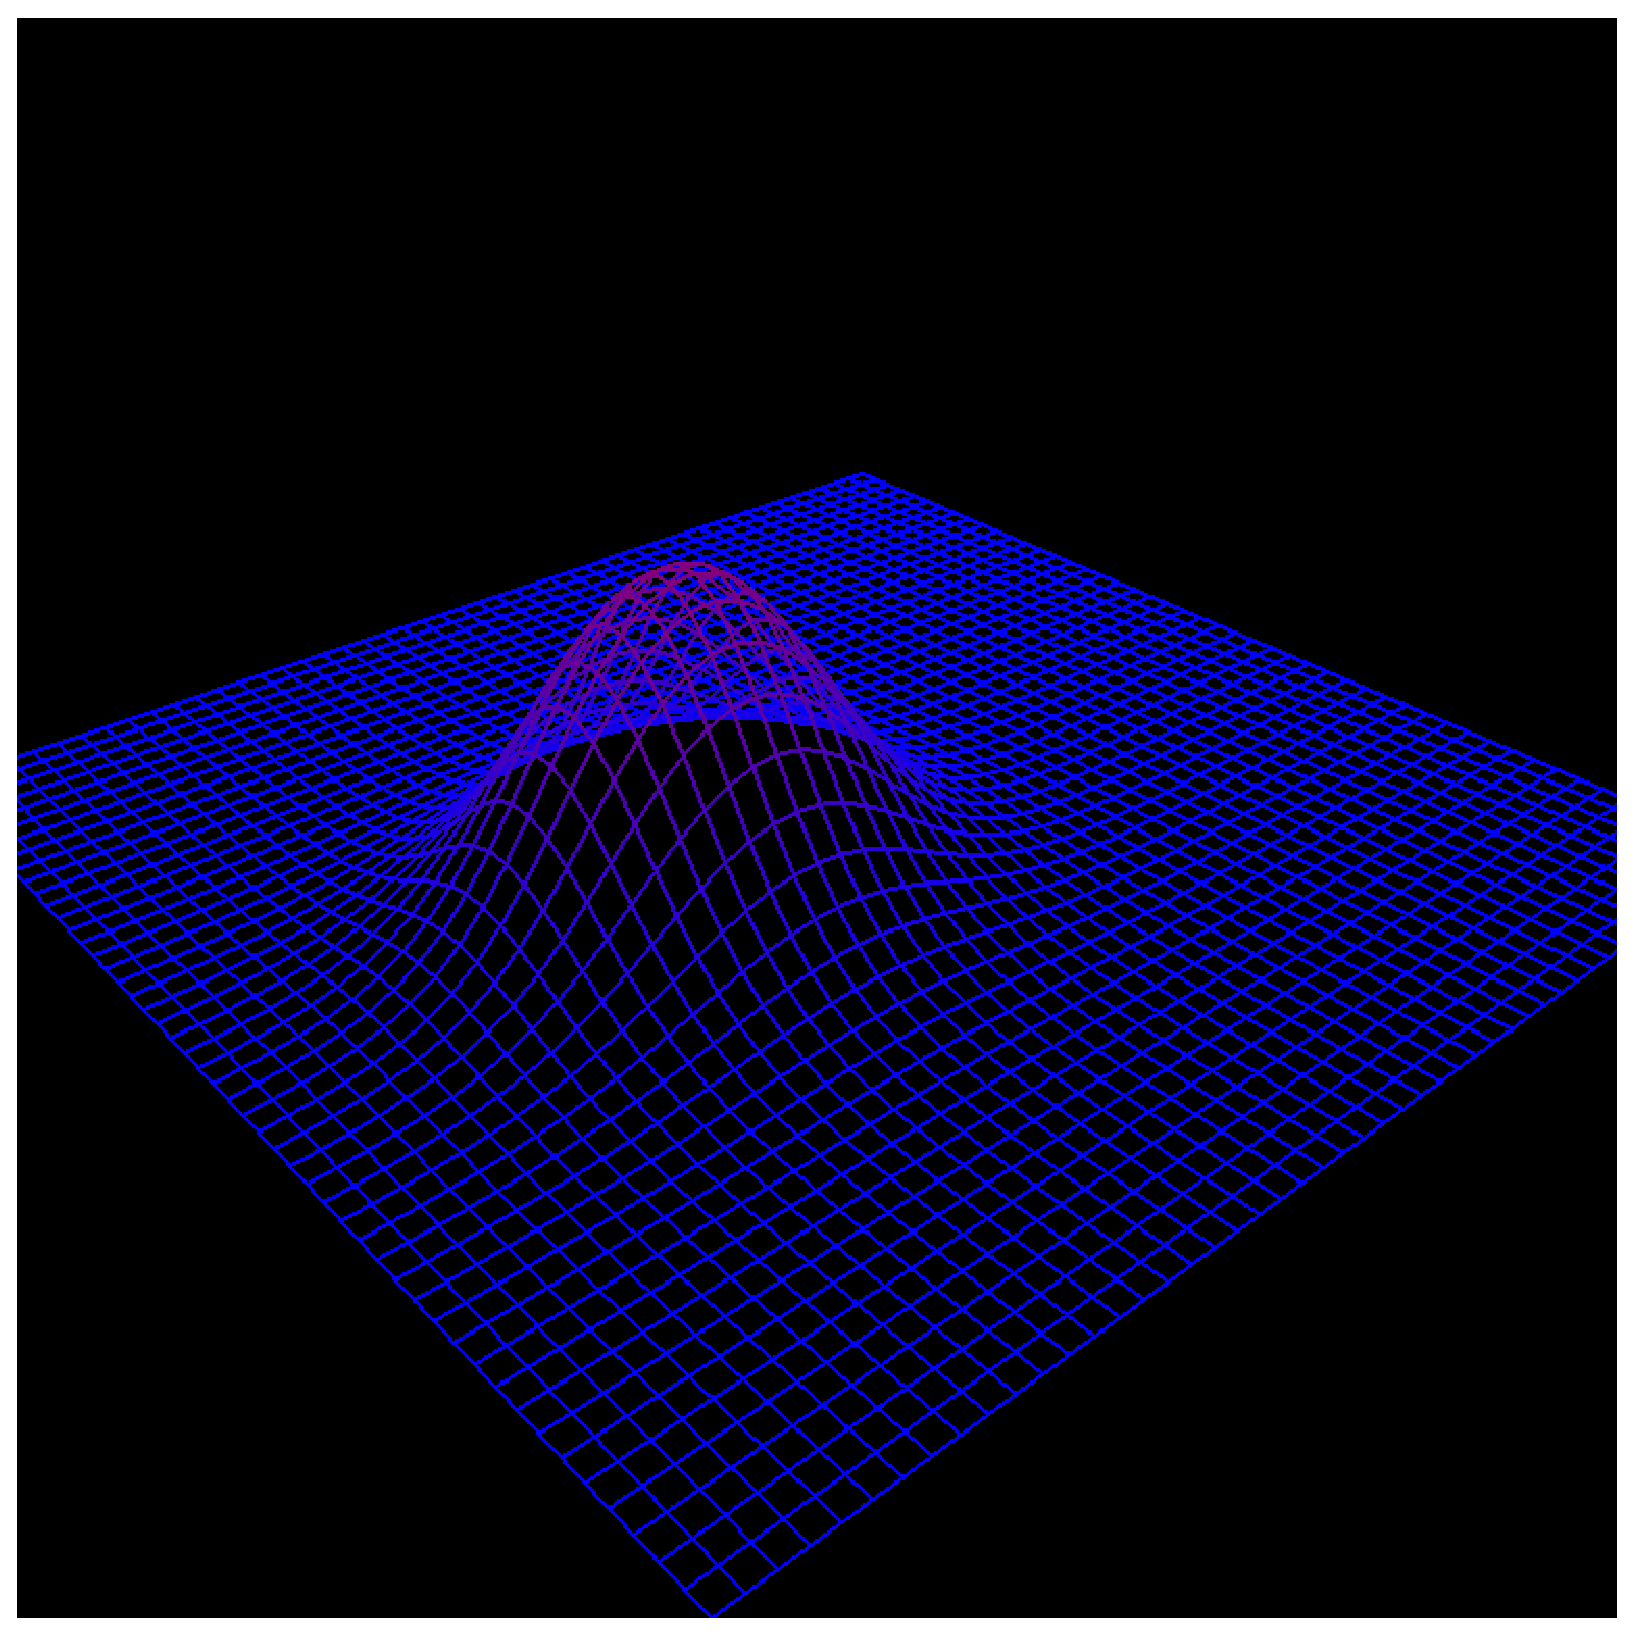
\includegraphics[scale=0.33]{im1_imp}
\parbox{4in}{\emph{\caption{$T_b=0$, $t_{end}=0.1$, 100 kroków czasowych, metoda implicite, początkowa wartość to ``wyspa'' wysokich temperatur na środku.
Ten krok czasowy to $t=0.005$, rozwiązanie jest ciągłe i pokrywa się z przypuszczeniami co do poprawnego zachowania}}}
\end{center}
\end{figure}
\begin{figure}[ht]
\begin{center}
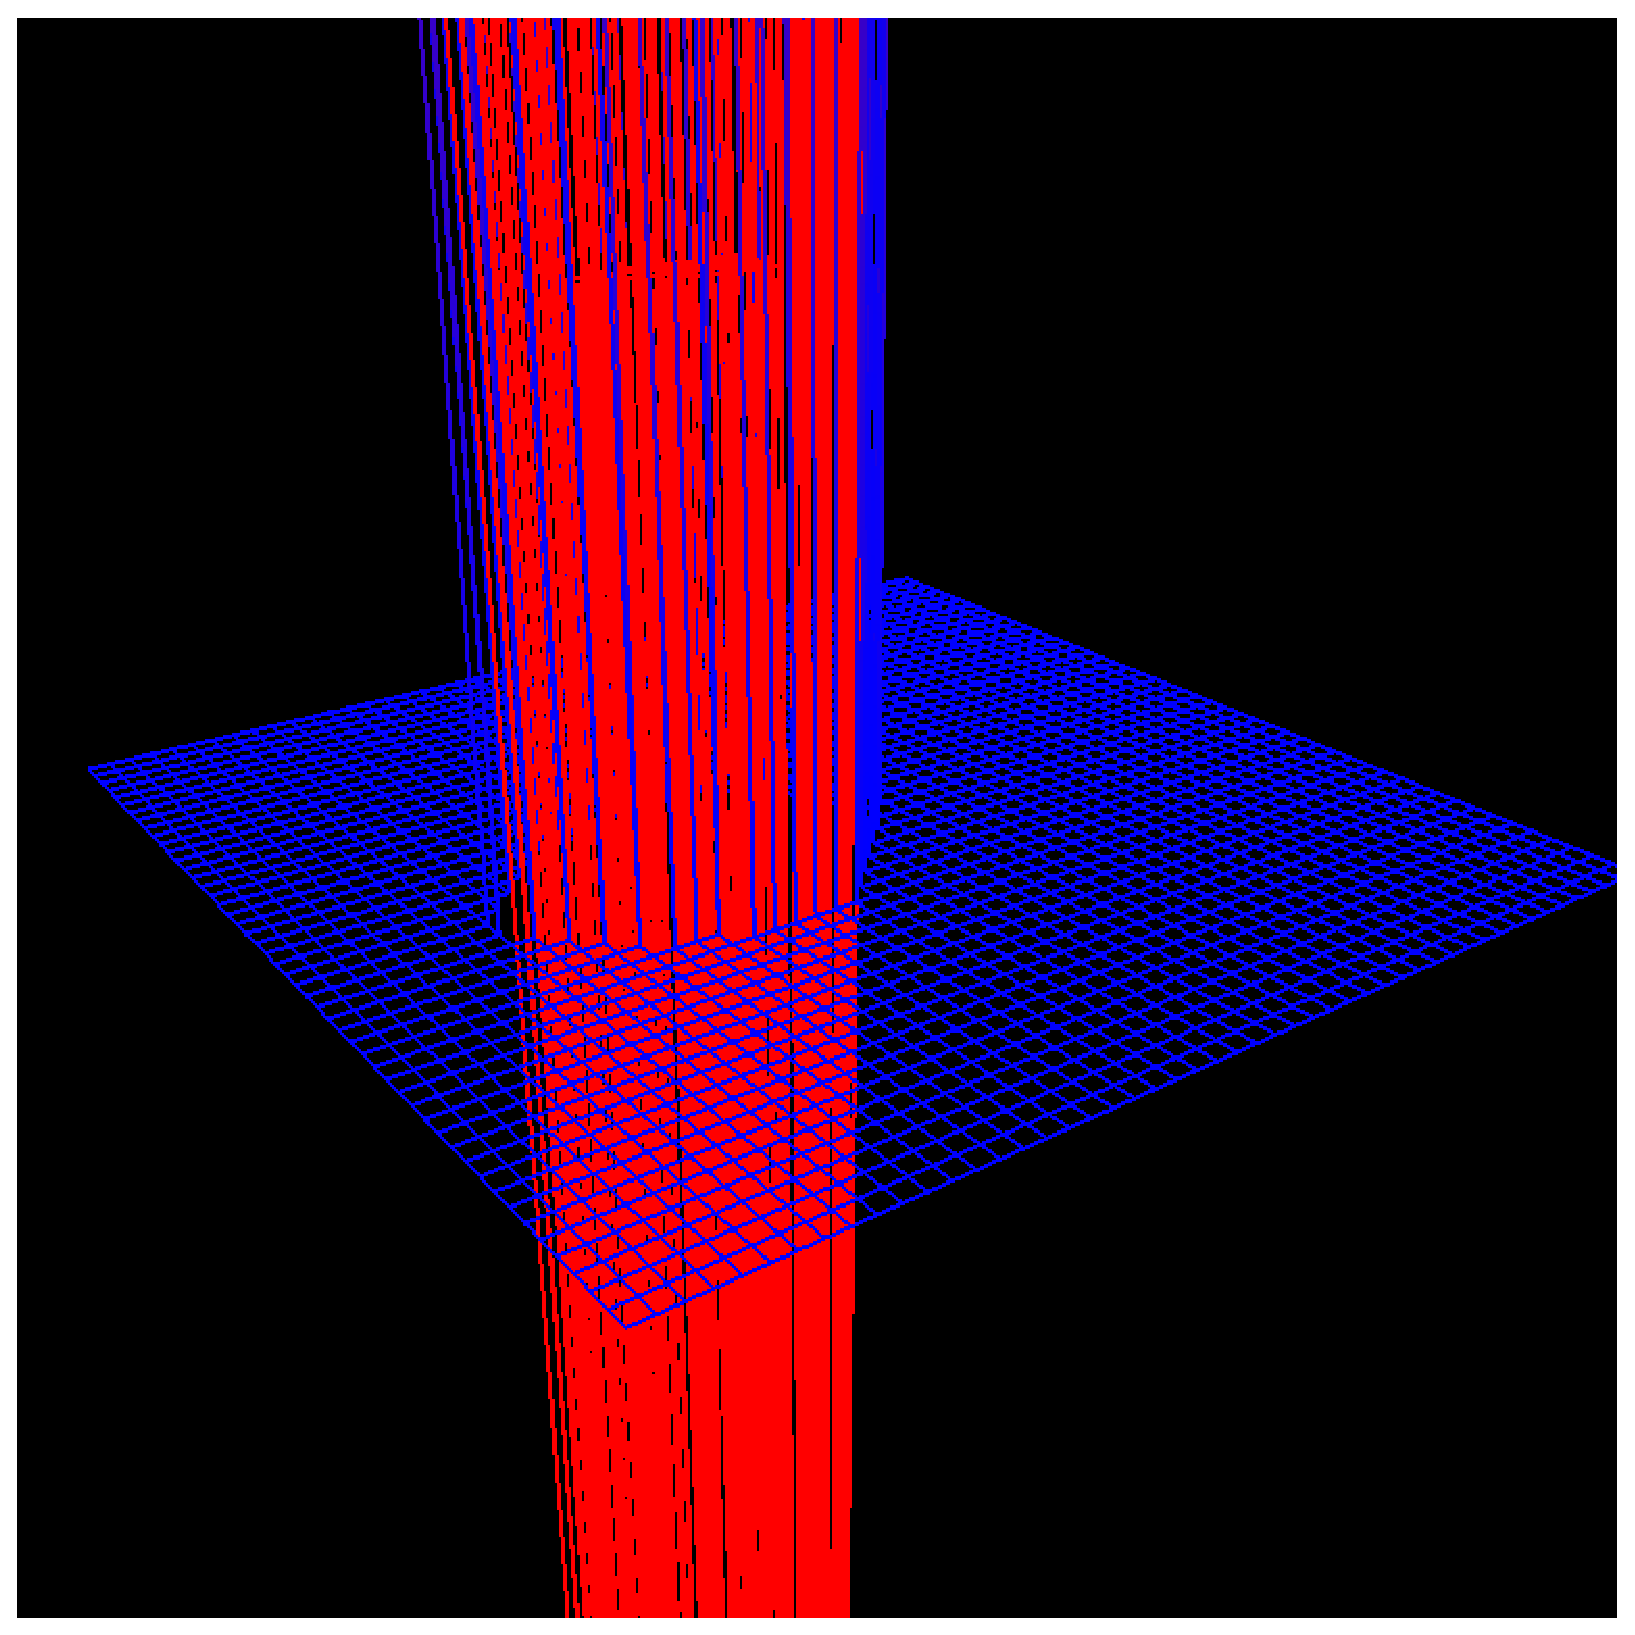
\includegraphics[scale=0.33]{im1_exp}
\parbox{4in}{\emph{\caption{$T_b=0$, $t_{end}=0.1$, 100 kroków czasowych, metoda explicite, początkowa wartość to ``wyspa'' wysokich temperatur na środku.
Ten krok czasowy to $t=0.005$, mimo tego samego zadania problemu co w poprzednim rysunku, pojawiają się ogromne błędy. obliczeniowe i bezsensowne wyniki.}}}
\end{center}
\end{figure}
\begin{figure}[ht]
\begin{center}
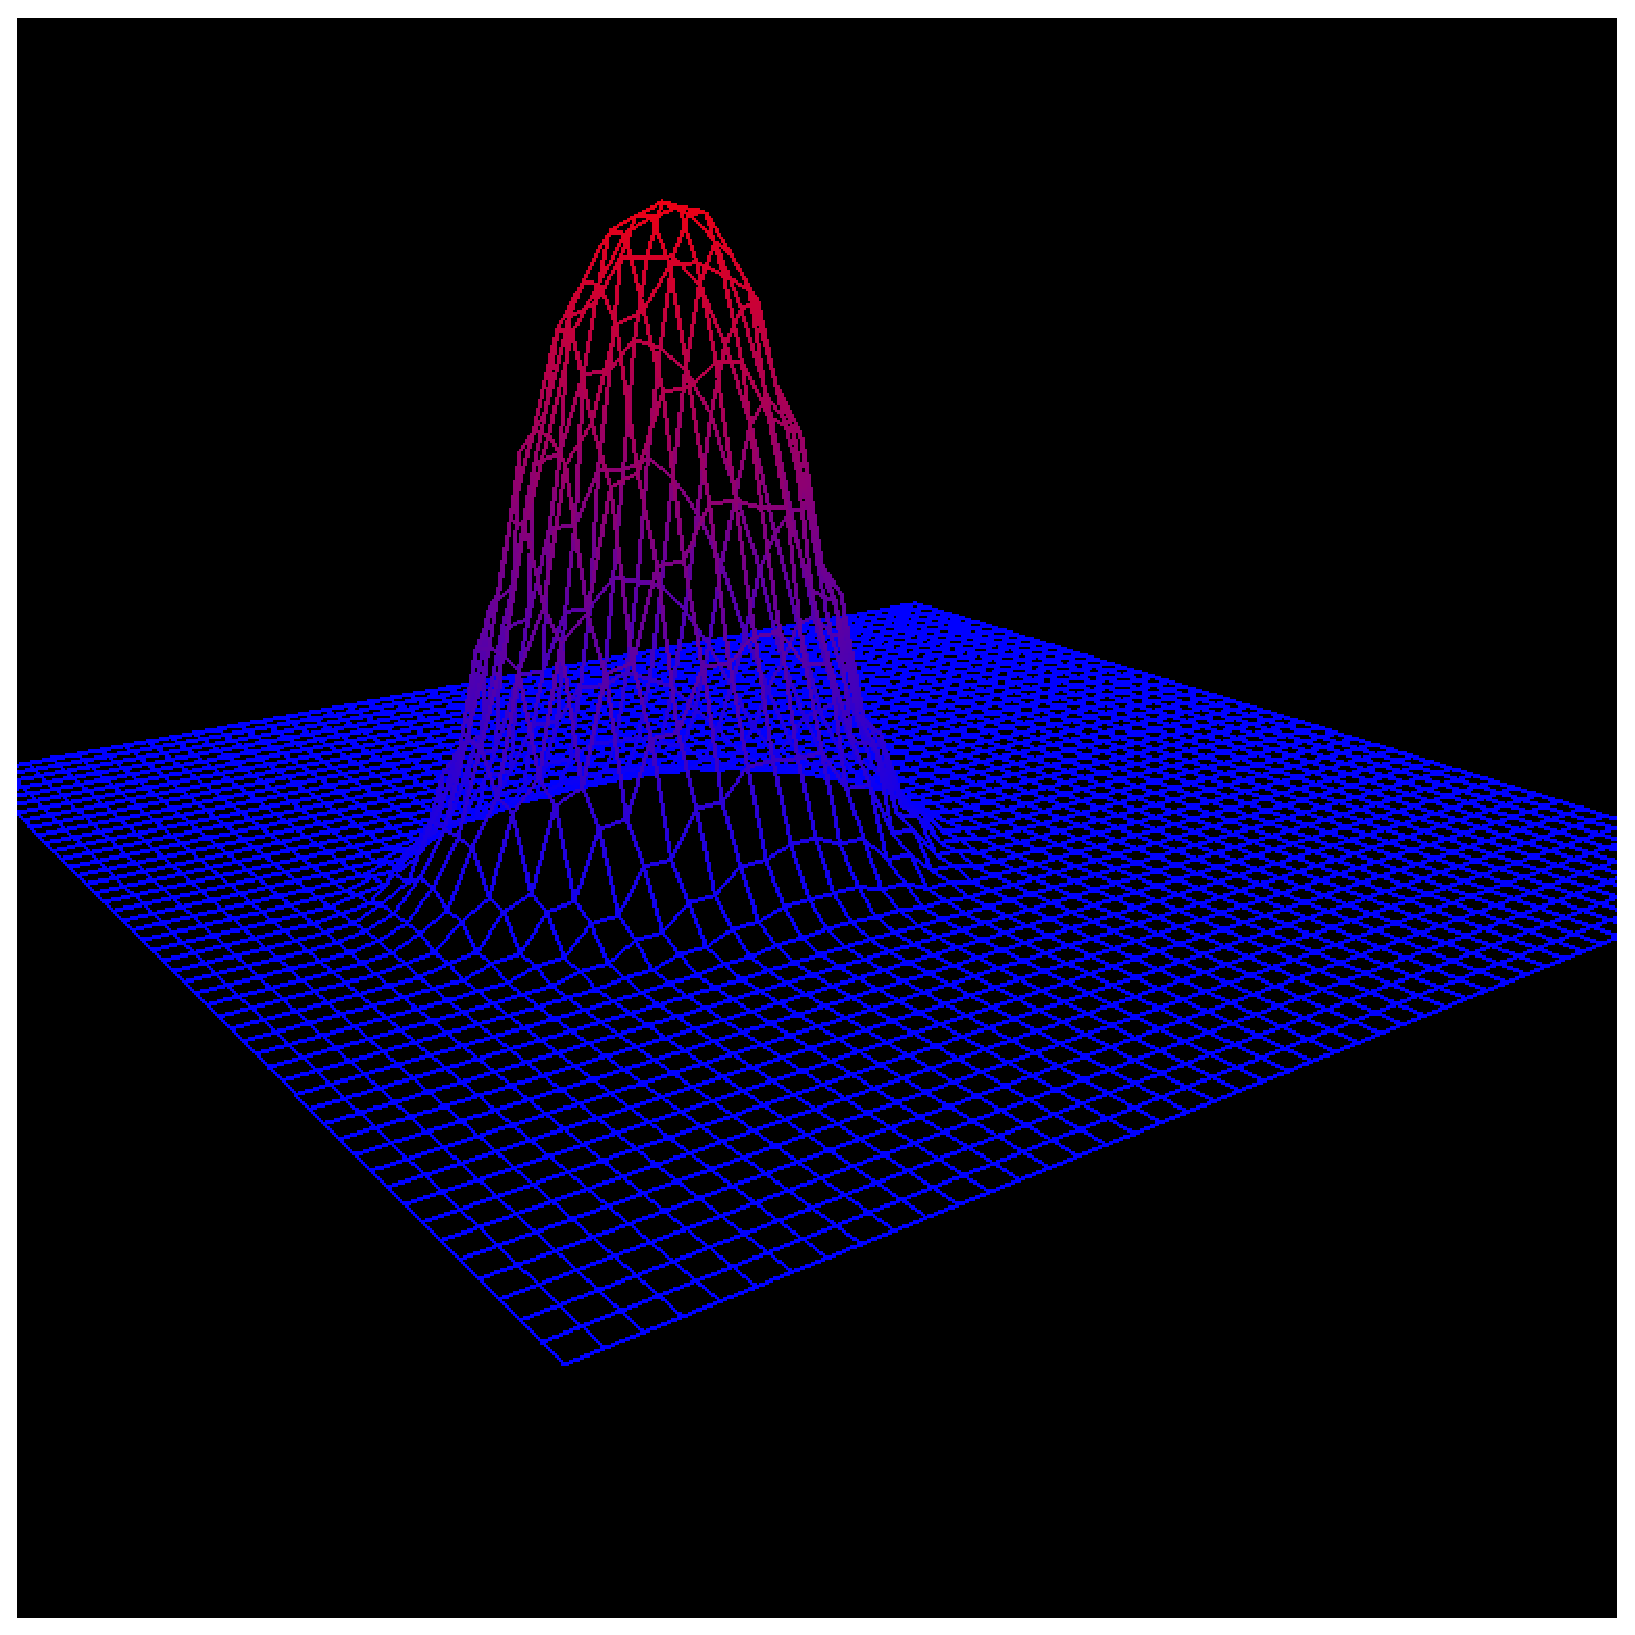
\includegraphics[scale=0.33]{im1_exp_fix}
\parbox{4in}{\emph{\caption{$T_b=0$, $t_{end}=0.1$, 1000 kroków czasowych, metoda explicite, początkowa wartość to ``wyspa'' wysokich temperatur na środku.
Ten krok czasowy to $t=0.005$, teraz wynik jest sensowny, ale nie jest tak ciągły jak rozwiązanie implicite, wydłużył się także znacznie czas obliczeń - 
choć wciąż jest wielokrotnie mniejszy od czasu obliczeń metody implicite. Uzyskanie tak samo ciągłego rozwiązania niweluje tę różnicę czasową. Jak widać, rozwiązanie implicite
jest znacznie bardziej stabilne}}}
\end{center}
\end{figure}
\begin{figure}[ht]
\begin{center}
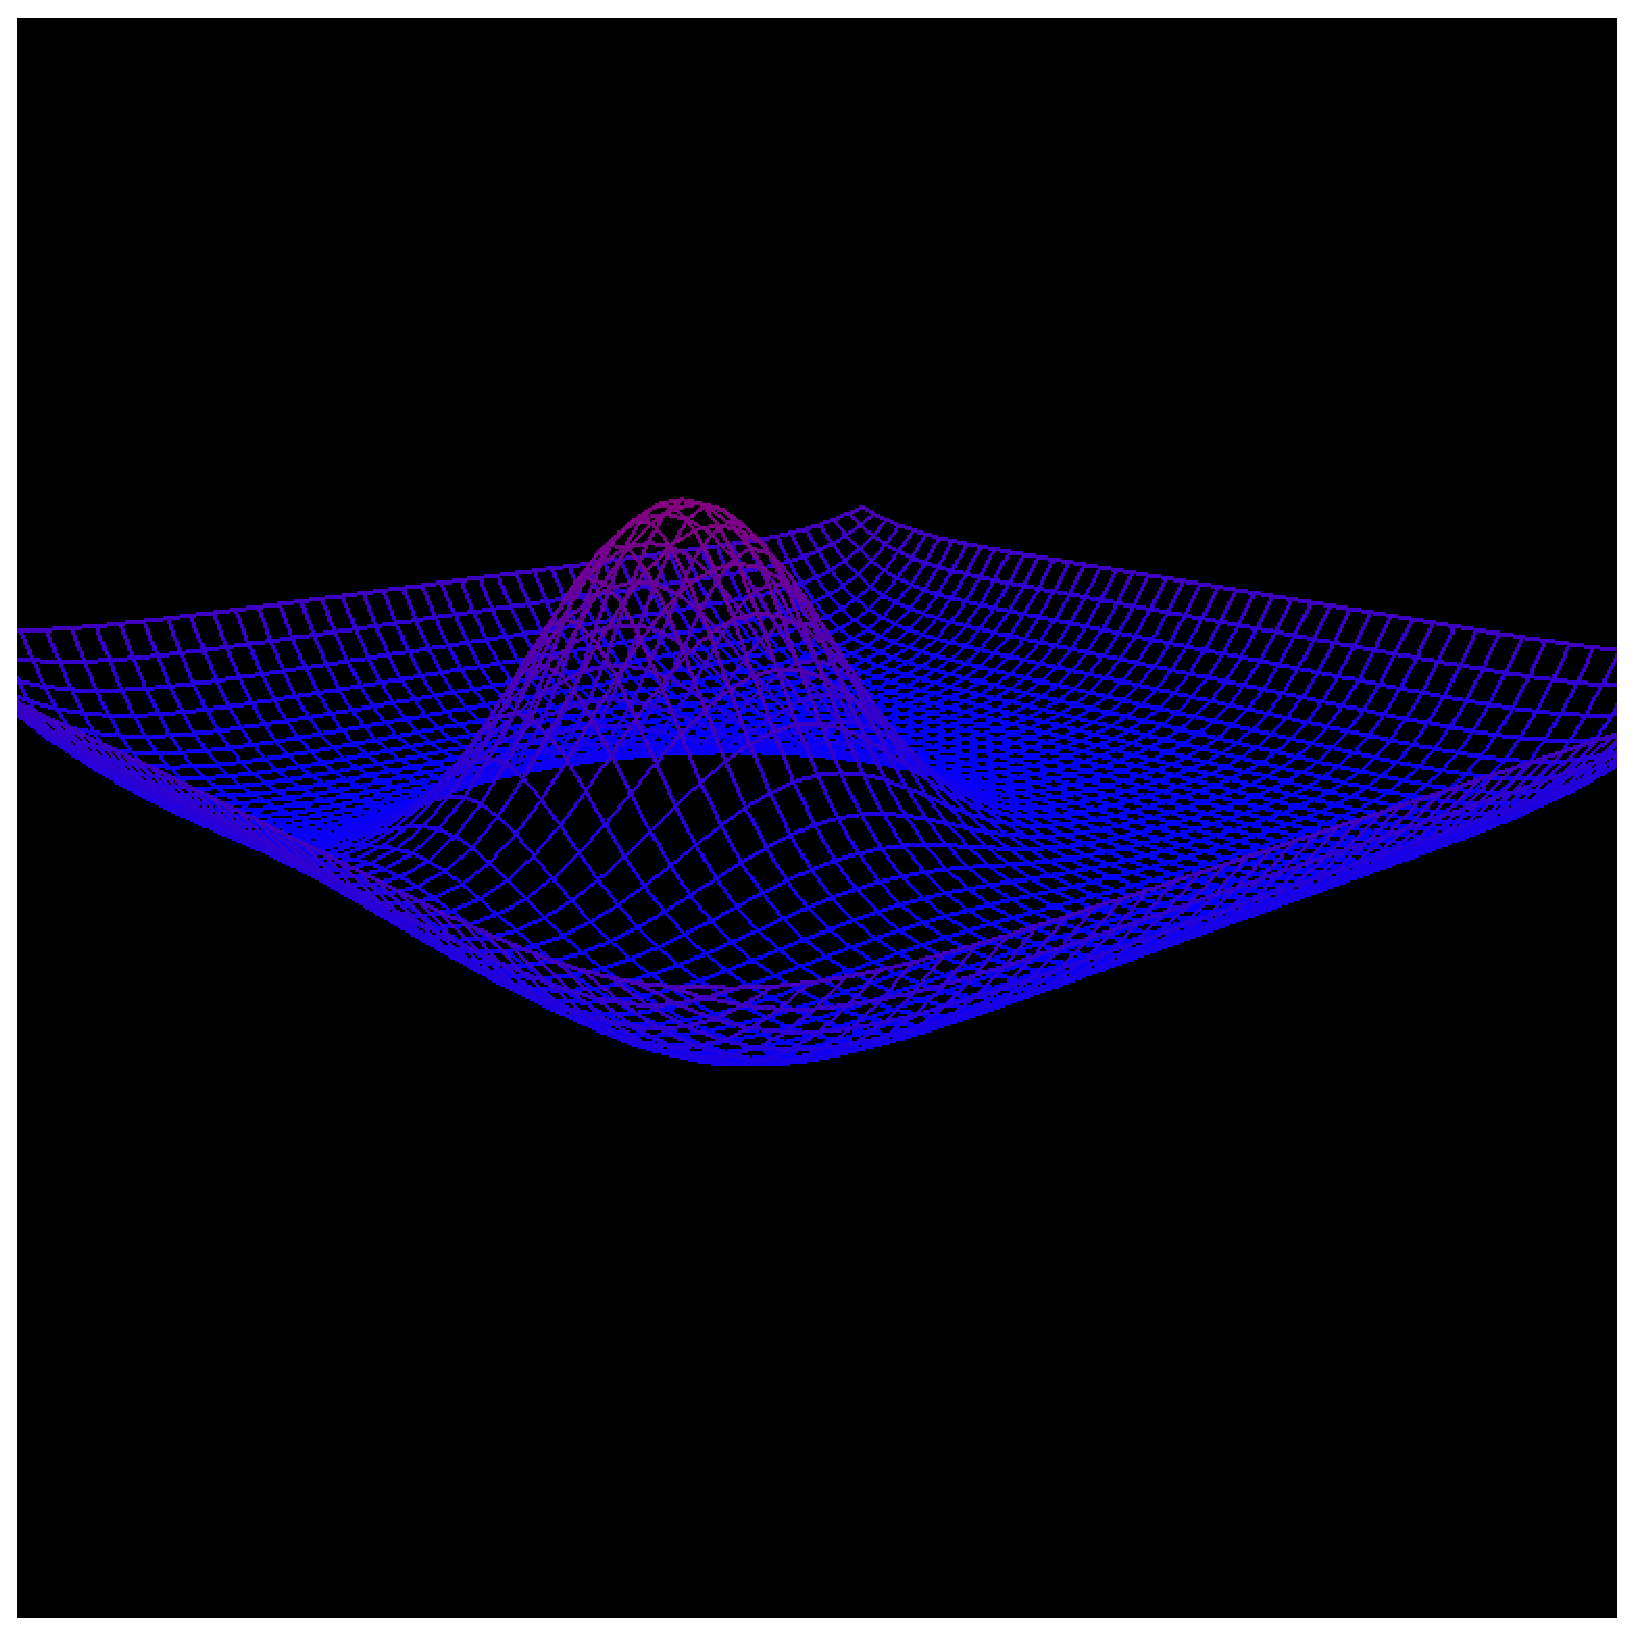
\includegraphics[scale=0.33]{im2_imp}
\parbox{4in}{\emph{\caption{$T_b=30$, $t_{end}=0.1$, 100 kroków czasowych, metoda implicite, początkowa wartość to ``wyspa'' wysokich temperatur na środku.
Ten krok czasowy to $t=0.005$, rozwiązanie jest ciągłe i pokrywa się z przypuszczeniami co do poprawnego zachowania}}}
\end{center}
\end{figure}
\begin{figure}[ht]
\begin{center}
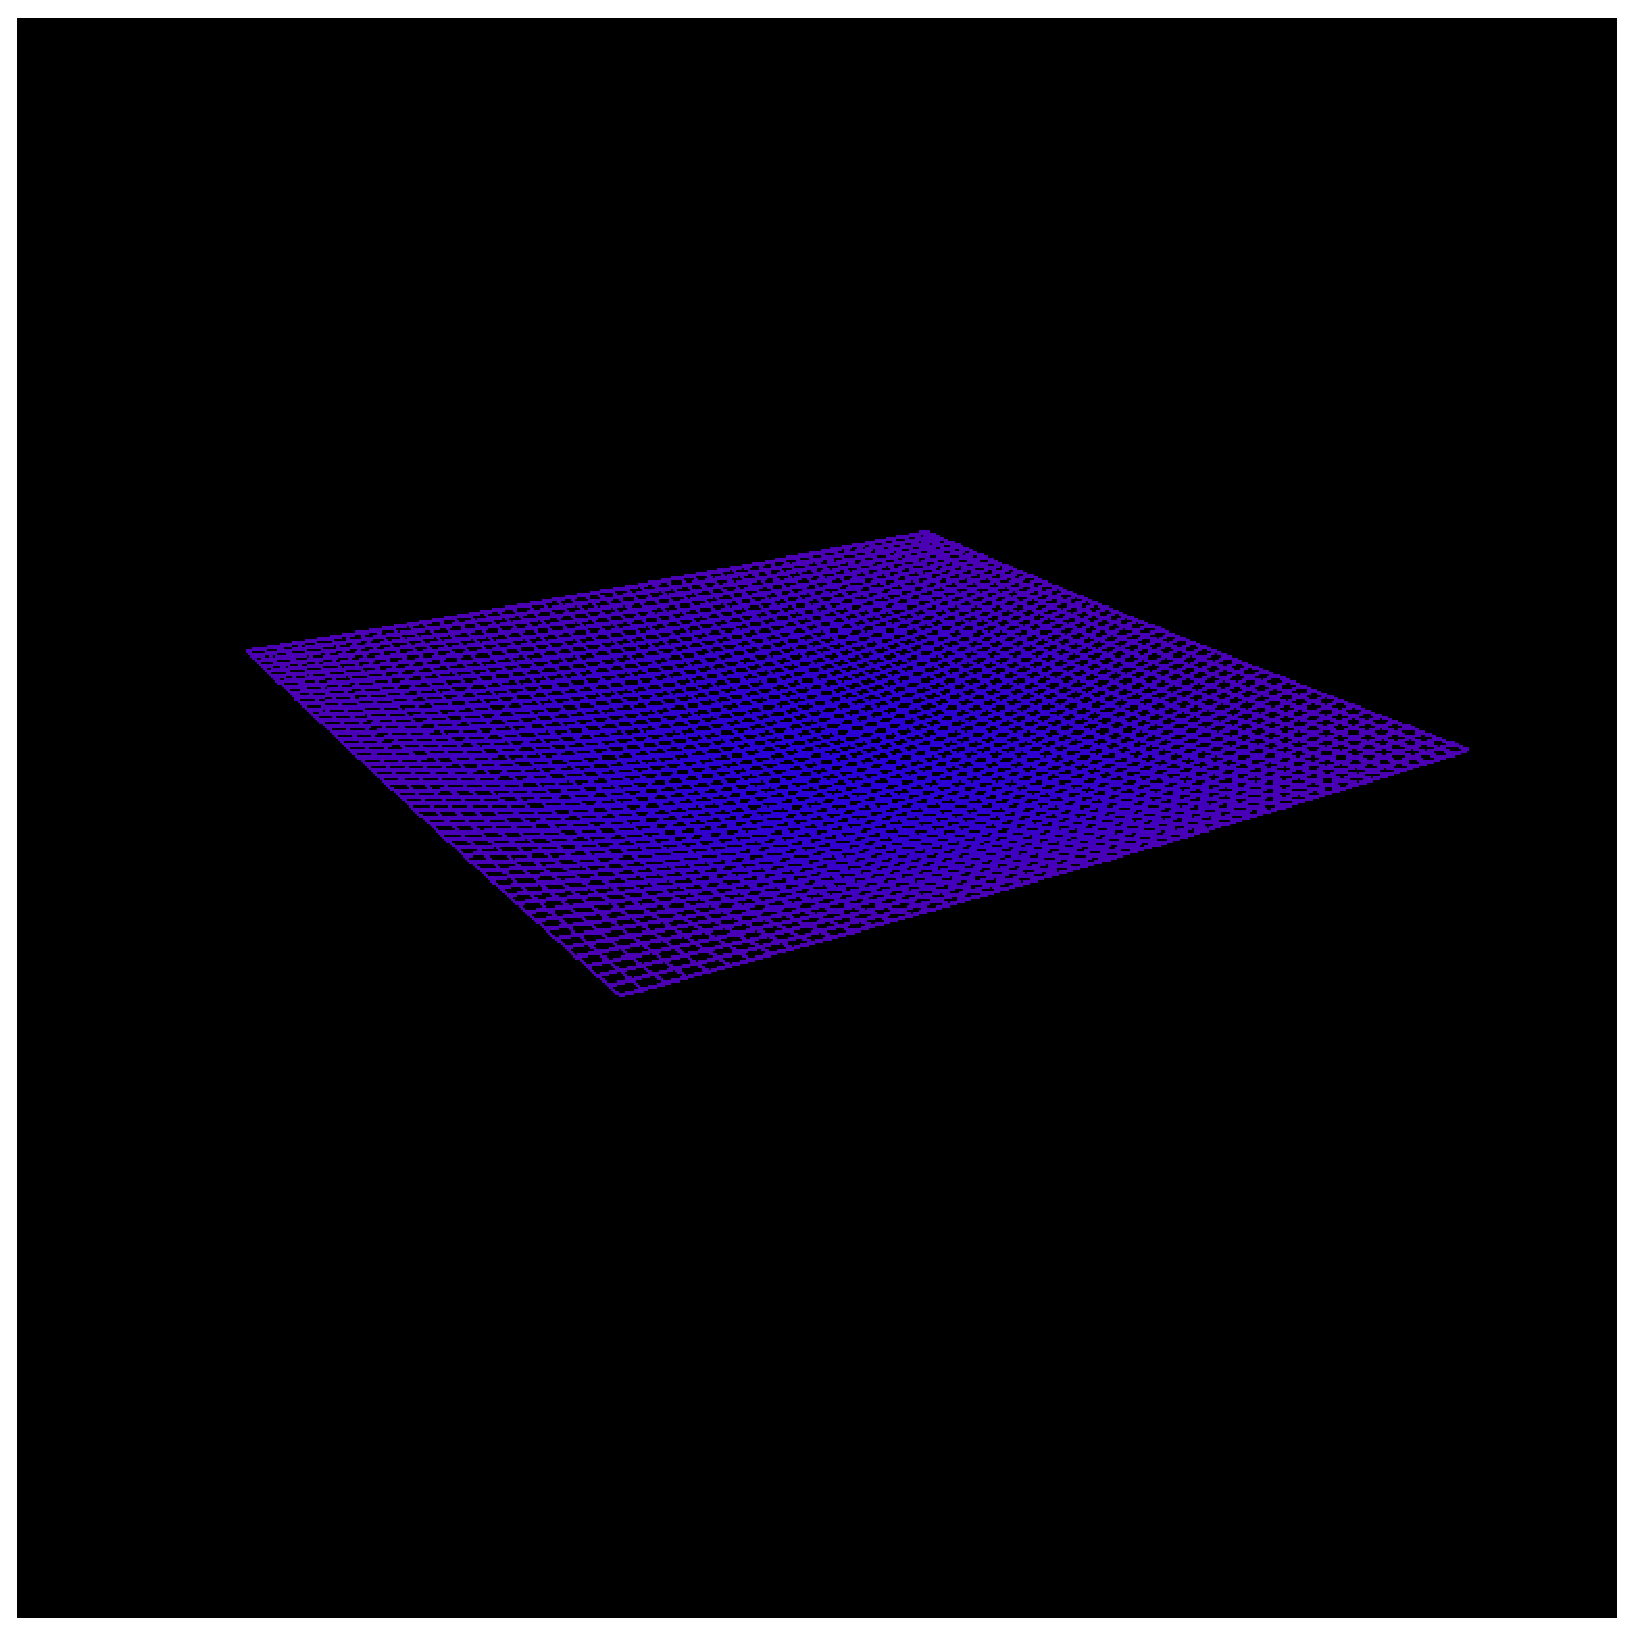
\includegraphics[scale=0.33]{im3_imp}
\parbox{4in}{\emph{\caption{$T_b=30$, $t_{end}=0.05$, 50 kroków czasowych, metoda implicite, ten sam problem co wcześniej, krok końcowy.
Widać zbliżenie płytki do temperatury na brzegu.}}}
\end{center}
\end{figure}
\end{document}
